\chapter{Assesment of Transcriptional Induction, Expression, and Subcellular Localisation of Bovine IFITs in the Context of RSV} \label{Assesment of Transcriptional Induction, Expression, and Subcellular Localisation of Bovine IFITs in the Context of RSV}
\section{Introduction and Aims} \label{Introduction and Aims}
\textbf{Half page intro:}
about cross species interaction + question about lab attenuated or not the brsv stuff
\textbf{Half page aims:}
We hypothesised both human and bovine IFITs to be induced by human and bovine RSV infection. We aimed to systematically test this by initially confirming that our model cell lines are capable of IFIT induction following the treatment of known innate immune system activators such as interferons, LPS, and poly I:C. We would then assess the IFIT induction during human and bovine RSV infection using a range of viral concentration and end assay time points. Lastly, we would validate this data in more physiologically relevant cell lines as well as using omics approaches.

\section{Results} \label{Results}

\subsubsection{MDKB responses to hRSV} \label{MDKB responses to hRSV}
Describe data: \newline
asdasdas

Data show that ultracentrifugation purified hRSV causes no response in terms of bIFIT induction. Infection with normally purified virus does not cause induction either but hints at downregulation actually.

\begin{figure}
    \centering
    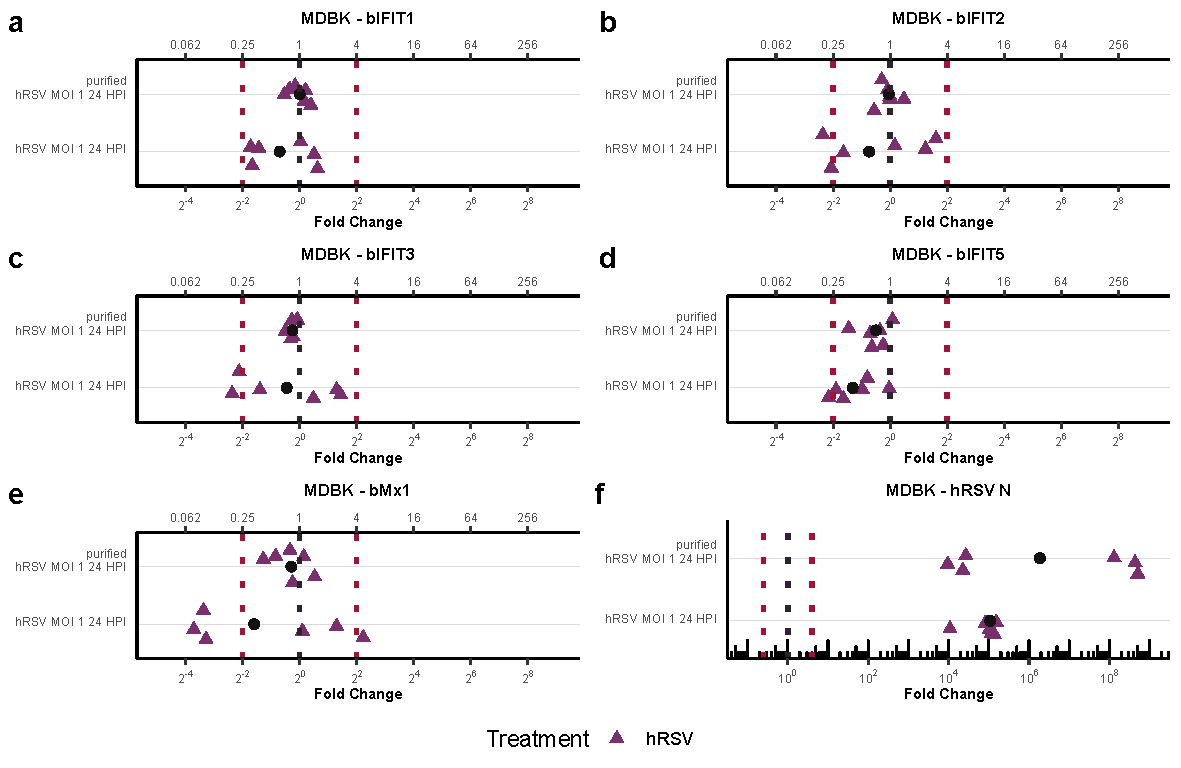
\includegraphics[width=1\linewidth]{07. Chapter 2//Figs/07. mdbk_hrsv_plots.pdf}
    \caption[bIFIT responses to hRSV infection in MDBK.]{\textbf{bIFIT responses to hRSV infection in MDBK.} asdf asdf asdf asdf asdf asdf asdf asdf asdf }
    \label{bIFIT responses to hRSV infection in MDBK}
\end{figure}



% add this to the next chapter

\subsubsection{Responses of Human Cell Lines to bRSV} \label{Responses of Human Cell Lines to bRSV}
How were viruses harvested and cells infected \newline
Justify moi and timepoints

\begin{figure}
    \centering
    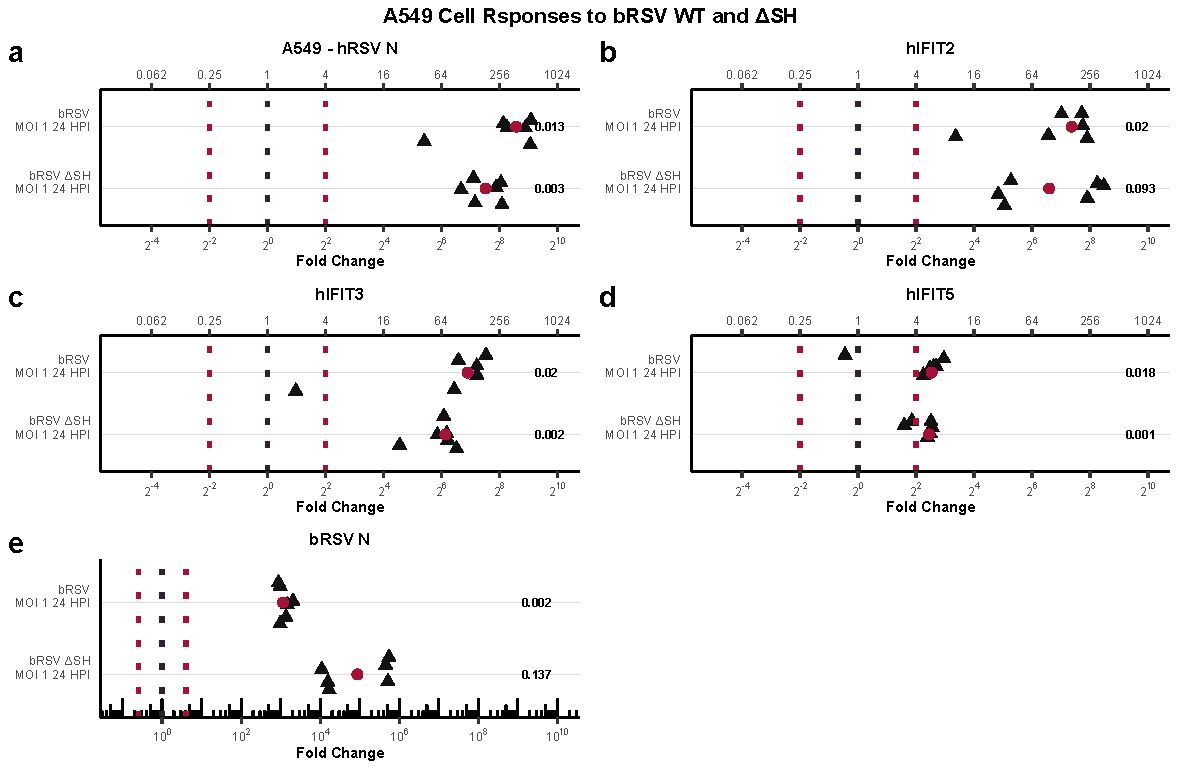
\includegraphics[width=1\linewidth]{06. Chapter 1/Figs/01. Induction/07. a549_brsv_moi1.pdf}
    \caption[Responses of A549 to bRSV WT and dSH.]{\textbf{Responses of A549 to bRSV WT and dSH.} Some filler text afterwards to not to forget.}
    \label{Responses of A549 to bRSV WT and dSH.}
\end{figure}

Describe data: \newline
asdasdasd \newline
Infection cells with WT bRSV induces IFITs more than infection with hRSV.  Infection with mutant bRSV viruses (at normal and low MOI) induces human IFITs but IFIT5, which is only responsive to MOI 1 dSH bRSV and MOI 0.001 dNS1/2 bRSV.

The low MOI infection causing induction are interesting as low MOI hRSV did not cause induction. Maybe bRSV is more potent of A549 cells?

\begin{figure}
    \centering
    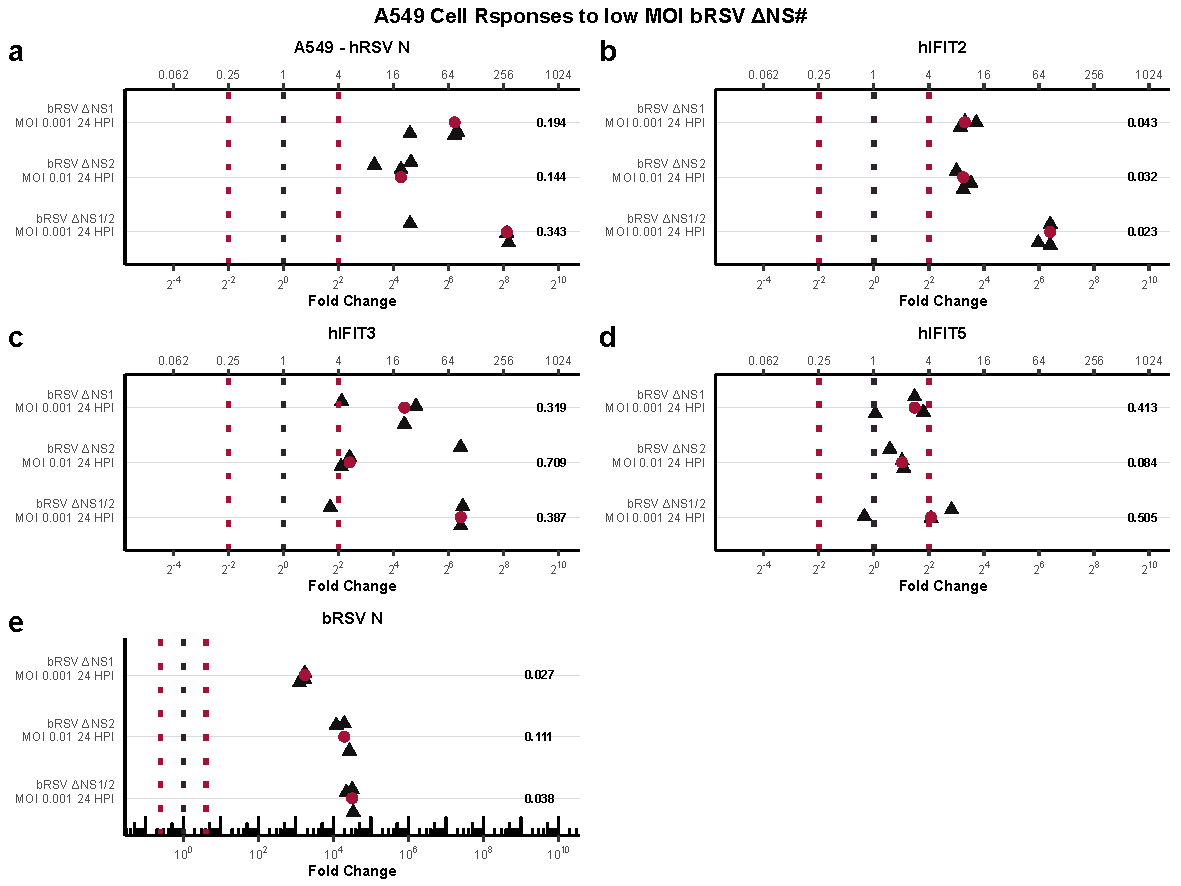
\includegraphics[width=1\linewidth]{06. Chapter 1/Figs/01. Induction/08. a549_brsv_dns.pdf}
    \caption[Responses of A549 to bRSV dNSs.]{\textbf{Responses of A549 to bRSV dNSs.} Some filler text afterwards to not to forget.}
    \label{Responses of A549 to bRSV dNSs.}
\end{figure}

\begin{figure}
    \centering
    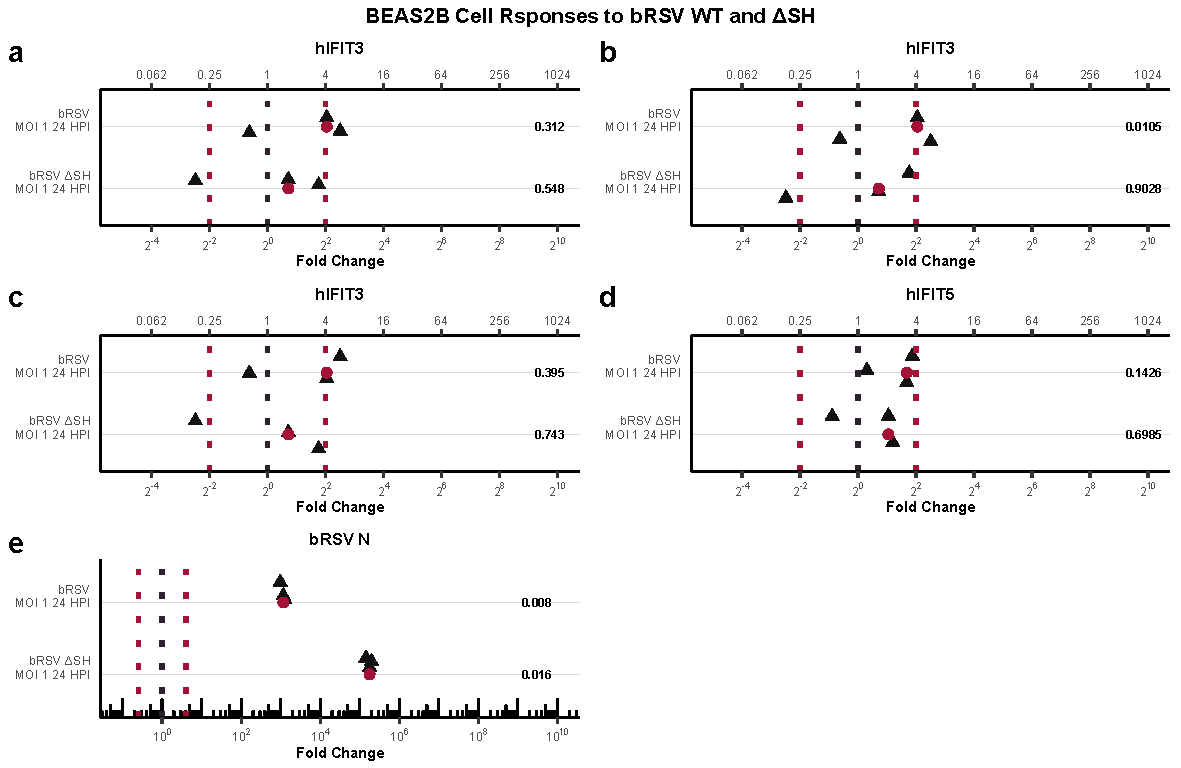
\includegraphics[width=1\linewidth]{06. Chapter 1/Figs/01. Induction/11. beas2b_brsv_moi1.pdf}
    \caption[BEAS-2B responses to bRSV WT and dSH.]{BEAS-2B responses to bRSV WT and dSH.}
    \label{BEAS-2B responses to bRSV WT and dSH.}
\end{figure}

\begin{figure}
    \centering
    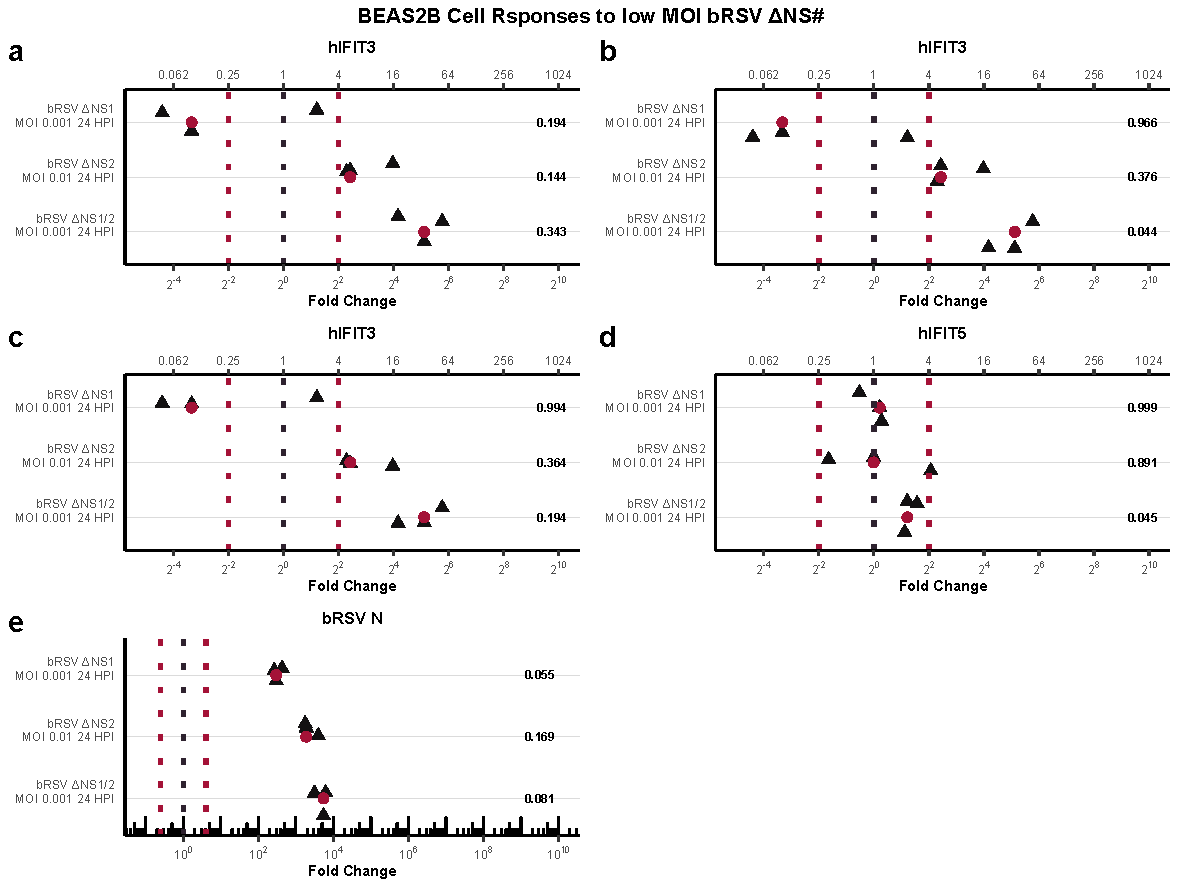
\includegraphics[width=1\linewidth]{06. Chapter 1/Figs/01. Induction/12. beas2b_brsv_dns.pdf}
    \caption[BEAS-2B responses to bRSV dNSs.]{BEAS-2B responses to bRSV dNSs.}
    \label{BEAS-2B responses to bRSV dNSs.}
\end{figure}

\section{Discussion} \label{Discussion}
Recap human \newline
Recap bovine \newline
Bovine rna seq studies